\section{Evaluation}

As stated before, we had problems with the runtime of our implementation on our available hardware.
Therefore, we could only test our implemenation and the general method of discovering patches based on their visual
discriminativness with very basic tests.\\
\\
One test we conducted was a discovery set $\mathcal{D}$ of 15 images containing busses, which we trained with a worldset 
$\mathcal{N}$ of 80.000 patches. The results for the best clusters based on SVM score are visualized in the figure below (top 5 patches), 
the rows show the results per iteration.\\
\\
\begin{figure}[h!]
\centering
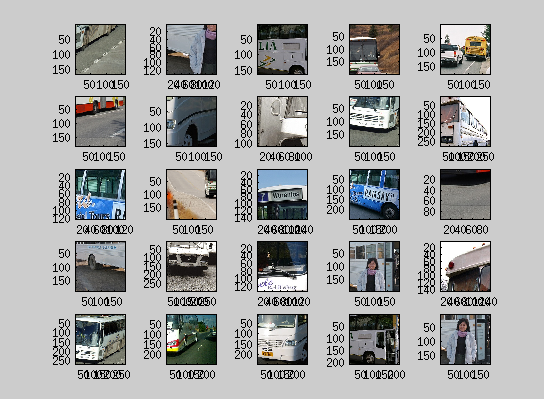
\includegraphics[width=0.9\textwidth]{figures/busses.png}
\caption{Per iteration results - Discriminative patches for busses}
\end{figure}
\\
As we can see, the top cluster is homogeneous with patches from different visual concepts (parts of busses, but also a person).
To prevent this, Singh et al. encorporated a method to clean up homogeneous cluster by finding what they called ``doublets'' \cite{Singh2012DiscPat}.\\
\\
Another test included a discovery set $\mathcal{D}$ of 10 images showing horses, trained with a natural worldset $\mathcal{N}$ of 40.000 patches.
The results for the best clusters based on the SVM score are shown below (top 5 patches), the rows again visualize the results per iteration.

\begin{figure}[h!]
\centering
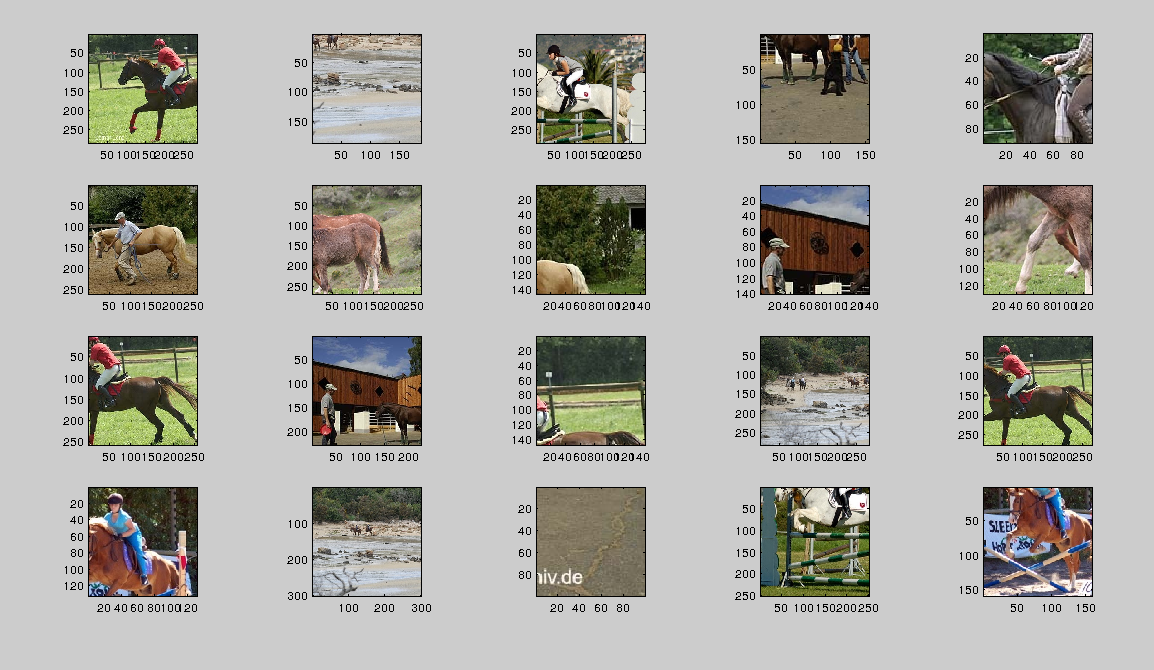
\includegraphics[width=0.9\textwidth]{figures/horses.png}
\caption{Per iteration results - Discriminative patches for horses}
\end{figure}

The SVM scores serves as an approximation for the \textit{purity} of the cluster, i.e. the percentage of
how many members of the cluster come from the same visual concept. To calculate the \textit{discriminativness}
of a patch, we have to calculate the ratio of firings of the patch on $\mathcal{D}$ and firings of the patch on $\mathcal{D} \cup \mathcal{N}$.
Since the results in Figure 1 and 2 are solely based on the SVM score or purity, this measure is missing in this visualization.